\chapter{Realizações}\label{chp:realizacoes}

\section{Calibração}

O processo de calibração do \textit{VCranium} foi complexo por abranger diversos conceitos e a sua aplicabilidade na plataforma do \textit{Unity} \cite{UnityOficial}. Decidimos fragmentar o problema e estudá-los separadamente:

\begin{description}
    \item[Rotação:] Realizado com o \textit{RVEC} de \textit{Rodrigues} de cada \textit{frame};
    \item[Translação:] Realizado com o \textit{TVEC} de \textit{Rodrigues} de cada \textit{frame};
    \item[\textit{Field of View}:] (\textit{FOV}) Calculado com as informações intrínsecas da calibração da câmera;
    \item[Distorção:] Calculado com as informações de distorção da calibração da câmera;
\end{description}

\subsection{Rotação}

A informação da rotação do modelo virtual do cérebro é adquirida da comunicação \textit{socket} com o servidor em \textit{Python}. Abaixo está estruturada o formato da mensagem enviada a cada iteração do computador para a aplicação:

\begin{figure}[ht]
    \centering
    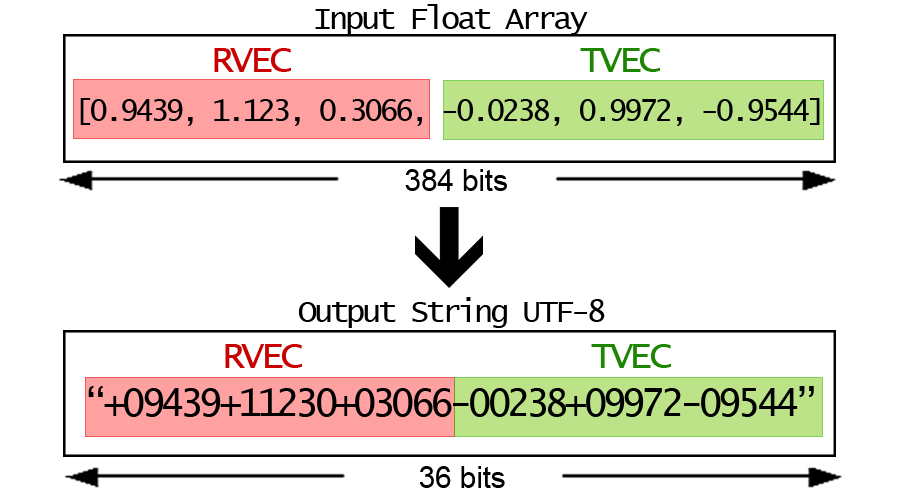
\includegraphics[width=.55\textwidth]{figuras/format rodrigues.png}
    \caption{Estrutura da mensagem via \textit{socket}. Fonte: Autor.}
    \label{fig:frodrigues}
\end{figure}

Um método foi implementado para a formatar cada mensagem gerada pela detecção da posição do marcador, transformando uma lista do \textit{Python} em uma \textit{string} com o formato de \textit{UTF-8}, como é mostrado no \textit{RVEC} da Figura \ref{fig:frodrigues}. Assim que a aplicação recebe os três números, eles representam o vetor de rotação com as coordenadas X, Y e Z, respectivamente. Para descobrirmos a magnitude da rotação neste eixo, deve-se calcular o módulo desse vetor de rotação, o resultado é dado em radianos.

\subsection{Translação}

Da mesma forma que a rotação, a translação é recebida do \textit{TVEC} da mensagem da Figura \ref{fig:frodrigues}. Nesta a informação é recebida em milímetros, portanto, devemos ajustar a escala da translação manualmente para corrigir a projeção do marcador no mundo virtual do \textit{Unity}. Com a rotação e translação completas, temos a calibração extrínseca da projeção. Assim como foi explicado no último relatório, a projeção deve estar visualmente boa, especialmente nas regiões centrais da tela, representado na Figura \ref{fig:Extrinsecos}.

\begin{figure}[ht]
    \centering
    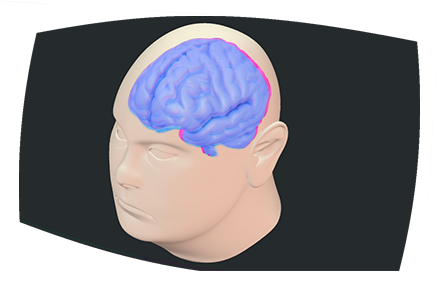
\includegraphics[width=.45\linewidth]{figuras/CalibExtr.png}
    \caption{Exemplo de sobreposição sem calibração intrínseca. Fonte: Autor.}
    \label{fig:Extrinsecos}
\end{figure}

\subsection{\textit{Field of View}}

O \textit{Field of View} (\textit{FOV}) é calculado da calibração da câmera com o \textit{chessboard} que calcula a distorção e os intrínsecos da câmera, nomeados respectivamente de \textit{DIST} e \textit{MTX}. Para determinar o \textit{FOV} da câmera observamos \textit{MTX}:

\begin{figure}[ht]
    \centering
    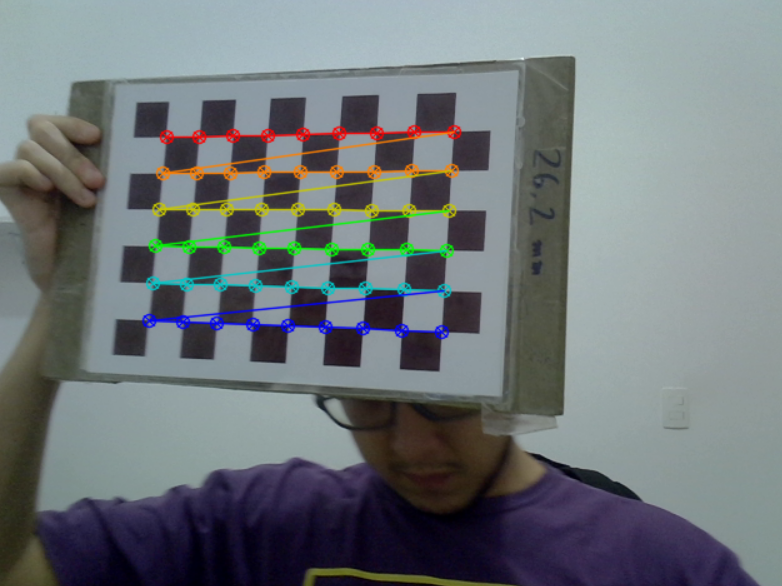
\includegraphics[width=.45\linewidth]{figuras/chessboard.png}
    \caption{Calibração dos intrínsecos da câmera com o \textit{chessboard}. Fonte: Autor.}
    \label{fig:chess_calib}
\end{figure}

\[ MTX = 
\begin{bmatrix}
    f_x & 0 & c_x \\    
    0 & f_y & c_y \\
    0 & 0 & 1
\end{bmatrix} \]

% DESCREVER PARAMETROS Sendo \(f_x\) o foco em X da câmera e
Utilizamos o \(f_x\) ou \(f_y\) da câmera e a informação das dimensões da imagem em \textit{pixels} para obter o \textit{FOV} em X e Y: 

\[
FOV_x = 2 \arctan \left( \dfrac{w}{2f_x} \right) ;
\ \ \ FOV_y = 2 \arctan \left( \dfrac{h}{2f_y} \right) 
\]
    
Sendo \(w\) e \(h\) a largura e a altura em \textit{pixels}, respectivamente. Não há diferença utilizar qualquer um dos dois, o \textit{Unity} suporta a configuração de ambos na câmera virtual, foi escolhido o \textit{FOV} em X pois é mais frequentemente usado na indústria. 
    
\subsection{Distorção}

Como foi mencionado no item anterior, a calibração também resulta em um vetor que modela as distorções de imagem da câmera. 


    % \section{Estudos de desenvolvimento Unity}
    
    % O \textit{Unity} foi o único programa em \textit{Unity} disponibilizado na documentação dos óculos, o projeto foi elaborado no \textit{Unity} 2017, mesmo com alguns alertas de incompatibilidade, o projeto pôde ser compilado com êxito e funcionou nos óculos. Novamente, a falta do suporte da \textit{EPSON} deixou incerto se era uma boa opção construir um aplicativo somente baseado na documentação disponível. Por isso, iniciamos novamente uma pesquisa sobre as ferramentas para suporte de AR nessa plataforma.
    
    % O \textit{Vuforia} foi o primeiro \textit{plugin} a ser testado no ambiente do \textit{Unity} \cite{Vuforia}. Em fevereiro de 2022, ele apresenta mais opções rastreio para AR, mas no início de 2021, no momento em que foi experimentado pela pesquisa, as opções eram de usar imagens e algumas formas 3D como marcadores para suas projeções. Foi testado a detecção de imagem com um pedaço da logo da \textit{Coca-cola\texttrademark} como alvo, a figura \ref{fig:vuforia-tests} ilustra os resultados.

% \begin{figure}[ht]
%     \centering
%     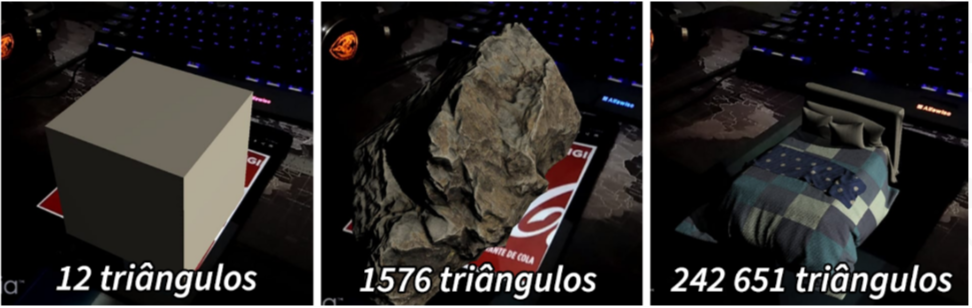
\includegraphics[width=.85\linewidth]{figuras/Vuforia.png}
%     \caption{Testes com diferentes modelos de diferentes complexidades, constatando performance acima de 15 quadros por segundo em todos os casos. Fonte: Autor.}
%     \label{fig:vuforia-tests}
% \end{figure}

% As formas de detecção tridimensionais não eram compatíveis com a detecção da posição da cabeça de um paciente, por isso esse recurso não foi testado. O \textit{Vuforia} é uma ferramenta que trabalha com \textit{Android} de \textit{API} 23 ou superior, infelizmente, também incompatível com o \textit{Moverio BT-350} que possui uma \textit{API} 22 e sem chances de atualização. Outras ferramentas foram encontradas como o \textit{Wikitude\texttrademark} que também era para \textit{API} 23 \cite{wikitudes}, porém uma outra ferramenta denominada \textit{ARFoundation} que estima a posição da face humana chamou a atenção por termos a oportunidade de criar uma demonstração da ideia final do projeto nos óculos \cite{arfoundation-docs}.

% \begin{figure}[ht]
%     \centering
%     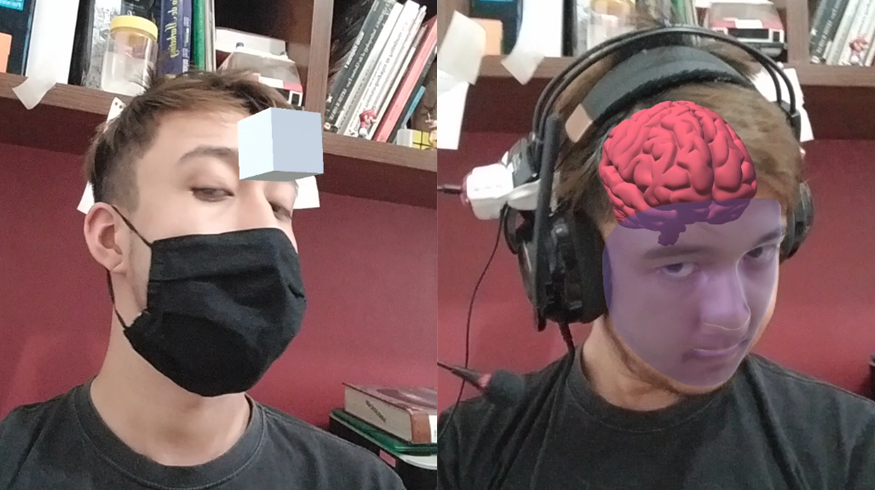
\includegraphics[width=.6\linewidth]{figuras/VCranium.png}
%     \caption{A primeira imagem foi o primeiro teste com a projeção de um cubo na região da testa. A segunda detalha a superfície estimada da face e a projeção do cérebro. Fonte: Autor.}
%     \label{fig:arfoundation}
% \end{figure}

% A instalação do \textit{ARFoundation} foi feita no \textit{Unity 2018} e apresentou compatibilidade com celulares de \textit{API 28} ou superior. Os testes consistiram em utilizar a posição da face encontrada pelo \textit{plugin} para projetar um objeto em referência a esses dados. A aplicação teve um ótimo resultado e foi possível apresentar o objetivo principal para professores e médicos da área pela aproximação visual dos testes com o resultado final esperado, visto na figura \ref{fig:arfoundation}. Nesse momento, criamos um nome fantasia para facilitar as apresentações do projeto: \textit{VCranium}.

% Retornando ao objetivo prático de encontrar um meio de desenvolver o projeto, concluímos que temos muitas opções disponíveis de desenvolvimento, mas sem muito suporte para o \textit{Moverio BT-350}. O \textit{Unity} foi escolhido para seguir a pesquisa pela sua facilidade de elaboração de cenários tridimensionais; compatibilidade com o sistema de outros óculos de \textit{AR} do mercado; e fornecimento de privilégios pela USP. Dessa maneira, podemos garantir que os próximos trabalhos que serão desenvolvidos, não dependem do equipamento que temos hoje, i.e, se futuramente precisarmos trocar para um óculos mais moderno, uma adaptação será feita e aproveitaremos o material produzido até o momento.

% Dado o histórico de testes do projeto, foi decidido prosseguir sem depender de \textit{plugins} e bibliotecas \textit{closed-source}, isso garantirá um maior controle do \textit{software} elaborado e também exigirá um estudo aprofundado do funcionamento dos algoritmos de visão computacional. Dessa forma, o projeto tem o potencial de ter um contato maior com problemas discretizados de programação, i.e, dúvidas específicas de funções empregadas. Isso facilita as pesquisas e levantamento de questões em seminário para os estudantes e professores dessa área de pesquisa na universidade.

% \section{Revisão bibliográfica}

% Aqui podemos analisar com mais atenção os artigos da literatura e suas diferentes soluções para sistemas de realidade aumentada aplicados em cirurgias. O trabalho que mais auxiliou a pesquisa foi uma revisão literária de aplicações em AR para neurocirurgias: \textit{"Enhancing Reality: A Systematic Review of Augmented Reality in Neuronavigation and Education"} \cite{enhancedvision}. Esse artigo faz uma breve apresentação da aplicabilidade de AR em ambiente cirúrgico e tabela as informações de doze pesquisas mostrando as patologias tratadas; descrição de método; e resultado da precisão da projeção em AR.

% Dentre as pesquisas descritas estava o artigo de Maruyama: \textit{Smart Glasses for Neurosurgical Navigation by Augmented Reality} \cite{Maruyama2018}. Sua equipe de pesquisadores construíram um sistema que utilizava os óculos \textit{Moverio BT-200}, um modelo que se assemelha muito com o que possuímos no laboratório, para auxiliar a visualização de tumores cerebrais em dois pacientes, além disso, foi também possível exibir a escalpe; o crânio; e os vasos da superfície do cérebro nos óculos.

% \begin{figure}[ht]
%     \centering
%     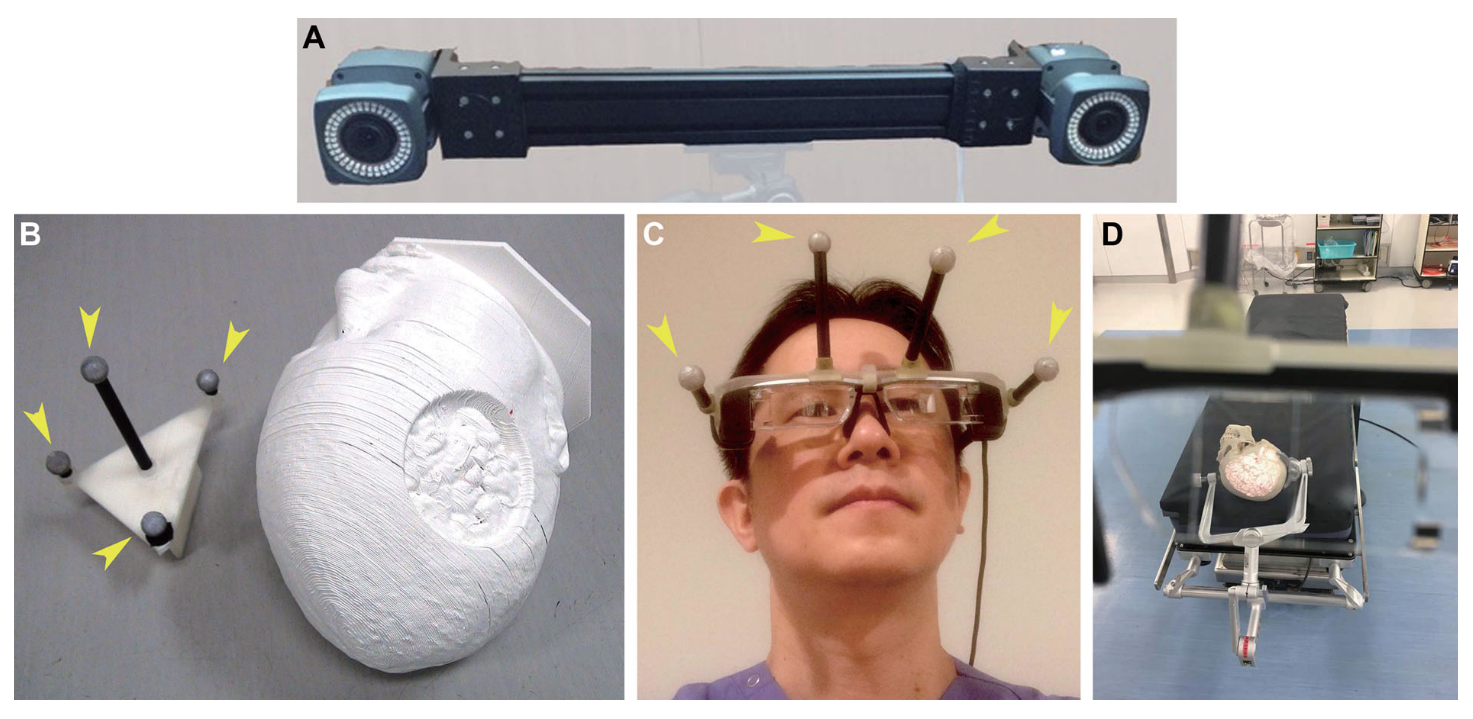
\includegraphics[width=.65\linewidth]{figuras/Maruyama.png}
%     \caption{(A) Duas câmeras para detectar movimento, (B) Marcadores para paciente, (C) Marcadores nos óculos, (D) Visualização nos óculos. Fonte: \cite{Maruyama2018}.}
%     \label{fig:maruyama}
% \end{figure}

% \begin{figure}
%     \centering
%     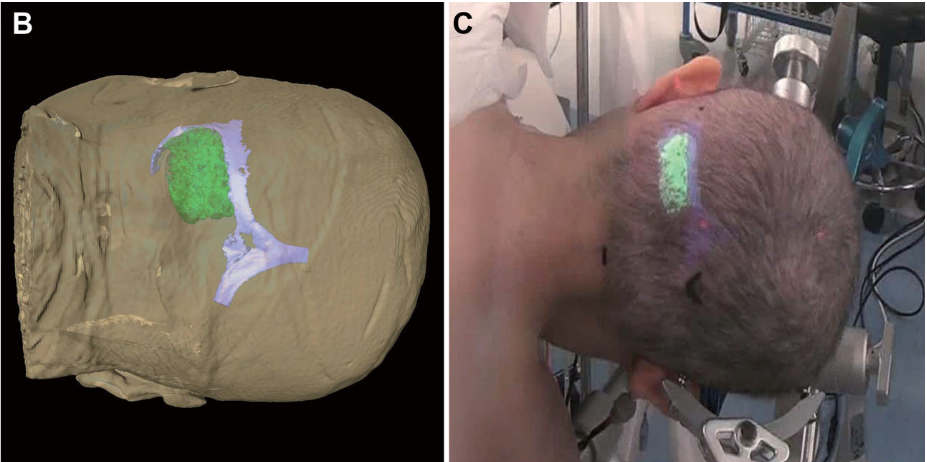
\includegraphics[width=.65\linewidth]{figuras/maruyama-overlay.png}
%     \caption{(B) Computação gráfica da reconstrução do cérebro do paciente, (C) Visualização em AR antes da incisão. Fonte: \cite{Maruyama2018}.}
%     \label{fig:maruyama-overlay}
% \end{figure}

% O método que o artigo utilizou apresentou a dinâmica da integração de componentes para uma arquitetura de um sistema AR: Empregar câmeras estereoscópicas para a detecção de marcadores nos óculos e na cabeça do paciente; relacionar com os dados da reconstrução 3D do cérebro; utilizar parâmetros da calibração; e fazer a exibição nos óculos. Por meio desse sistema, o resultado obtido é visto na figura \ref{fig:maruyama-overlay}.

% A precisão da projeção, segundo o artigo, foi de \(2.1 \pm  1.3\,mm\) com a mediana de \(1.8\) e a remoção total de \(5\) tumores com sucesso e sem complicações pós-operatórias. Além disso, o sistema tem uma interface de fácil utilização e conveniência para o médico, sendo possível desabilitar a projeção em qualquer momento da cirurgia, teve um custo menor que os sistemas de neuronavegação convencionais e, por fim, pode ser instalado em outros óculos de AR comerciais disponíveis, portanto, não se limitando ao seu modelo do \textit{Moverio} \cite{Maruyama2018}.

% Os resultados apresentados por essa pesquisa e a conjectura apresentada na seção anterior - aplicação baseado no \textit{Unity} para a compatibilidade com mais óculos do mercado - foram confirmados possíveis. Contudo, antes de simplesmente seguir os passos de Maruyama, decidimos fazer uma listagem das arquiteturas utilizadas em outros sistemas para tentar ponderar suas características para optarmos pela opção que mais atende as necessidades da pesquisa.

% \section{Elaboração do VCranium}\label{chp:criacao-vcranium} 

% \subsection{Arquitetura do Sistema}

% A definição da arquitetura do sistema é muito importante para configurar o seu funcionamento, estabelecer suas vantagens e desvantagens, e implicará como nós trabalhos em seu desenvolvimento. Para isso, a equipe realizou reuniões e debates para estabelecer uma solução que seja compatível para um período de seis meses e respeitando as medidas de prevenção por afastamento pela pandemia de COVID-19. Ainda assim, precisamos de uma arquitetura versátil e que objetiva facilitar a mudança de métodos de estimação a posição da projeção em AR. 

% Para tal, dividiremos o sistema em computador e óculos: O computador estima a posição da projeção e os óculos fazem a visualização nos olhos do usuário. Isso simplifica a mudança de método aplicado pelo computador, melhorando a recepção de novos algoritmos da equipe de estudos do laboratório. Esse sistema foi aplicado no artigo de Maruyama, que utilizou um \textit{software} de visualização médica e enviou os dados para os óculos que, por fim, fizeram a exibição do \textit{AR} utilizando o \textit{Unity} \cite{Maruyama2018}. Com a definição dos componentes da arquitetura, deve ser definido uma comunicação entre os dispositivos. Um exemplo da literatura foi o uso do computador para adquirir informações de sinais vitais de equipamentos médicos e o envio para os óculos via \textit{TCP/IP} (Protocolo de Controle de Transmissão / Protocolo de \textit{Internet}) \cite{Arpaia2021}.

% Utilizando o recurso de conexão \textit{wireless} dos óculos, podemos nos conectar com o computador via \textit{LAN} (Rede de área local). Na questão da estabilidade dessa conexão, em um espaço livre de obstáculos entre os óculos e a origem do sinal, a velocidade e latência são respectivamente \(100 \pm 10 \, Mbps\) e  \(15 \pm 10 \, ms\). Nota-se que com essa velocidade a conexão pode suportar a transmissão de vídeo e, portanto, harmoniza com a arquitetura mencionada anteriormente: O computador recebe imagens dos óculos e aplica algoritmos de visão computacional, e então retorna os dados com resultados para os óculos novamente.

% \begin{figure}[ht]
%     \centering
%     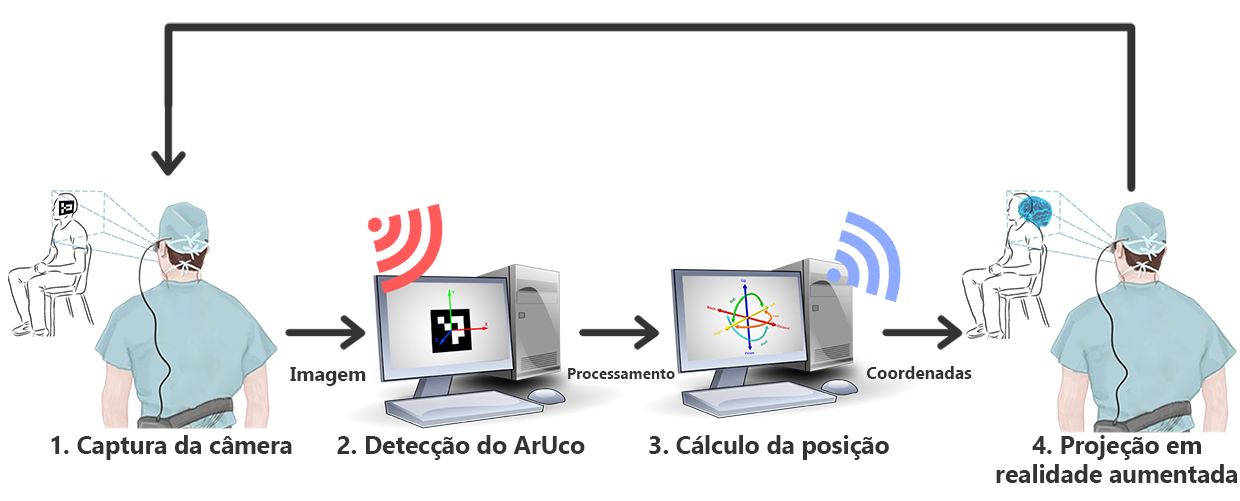
\includegraphics[width=.9\linewidth]{figuras/System schematic.png}
%     \caption{A figura representa o funcionamento do sistema. (1) Captura a imagem do paciente e envia para o computador. (2) Faz uma varredura na imagem e identifica o marcador ArUco. (3) Calcula a posição do marcador e envia as coordenadas para os óculos. (4) Recebe as informações e exibe a projeção para o usuário e então retorna para o passo 1. Fonte: Autor.}
%     \label{fig:arc}
% \end{figure}

% \subsection{Comunicação}

% A programação em C\# do sistema teve o desafio de conciliar a comunicação do computador programado em \textit{Python} com os óculos em plataforma \textit{Unity}. As pesquisas na \textit{web} demonstraram essa comunicação via \textit{TCP/IP} com a utilização de \textit{network sockets} \cite{socket-tutorial}. No entanto, o que precisava ser feito é a transmissão de vídeo em tempo real (\textit{video streaming}), essa ocasião é diferente do envio de uma mensagem de texto, que está na ordem de centenas de \textit{bytes}, uma única imagem pode carregar milhões de \textit{bytes} de informação.

% % \begin{figure}[ht]
% %     \centering
% %     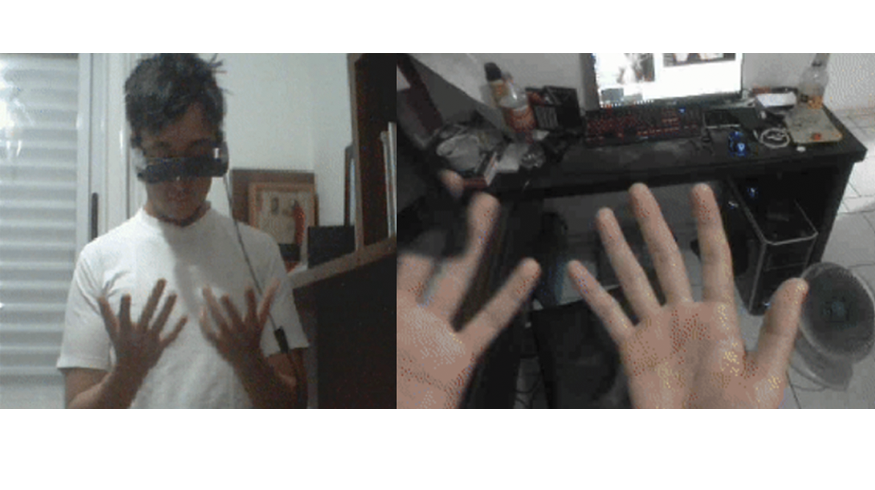
\includegraphics[width=.6\linewidth]{figuras/comm.png}
% %     \caption{Êxito da transmissão em tempo real das imagens dos óculos. Fonte: Autor.}
% %     \label{fig:communication}
% % \end{figure}

% Nos testes iniciais, a tentativa foi realizar o processo contínuo de capturar imagens e enviar dos dados via \textit{TCP} ao computador. Porém, ocasionalmente, a visualização da imagem era cortada horizontalmente, parecendo que "faltou um pedaço"\(\,\). Isso ocorre pois no processo de recepção de dados do \textit{socket}, a instrução de leitura não tem a informação do tamanho do arquivo a ser recebido da rede, i.e, o computador não pode interpretar onde é o fim da imagem, causando a renderização parcial das informações da foto, resultando em uma imagem defeituosa.

% \begin{figure}[ht]
%     \centering
%         \begin{subfigure}{.45\textwidth}
%             \centering
%             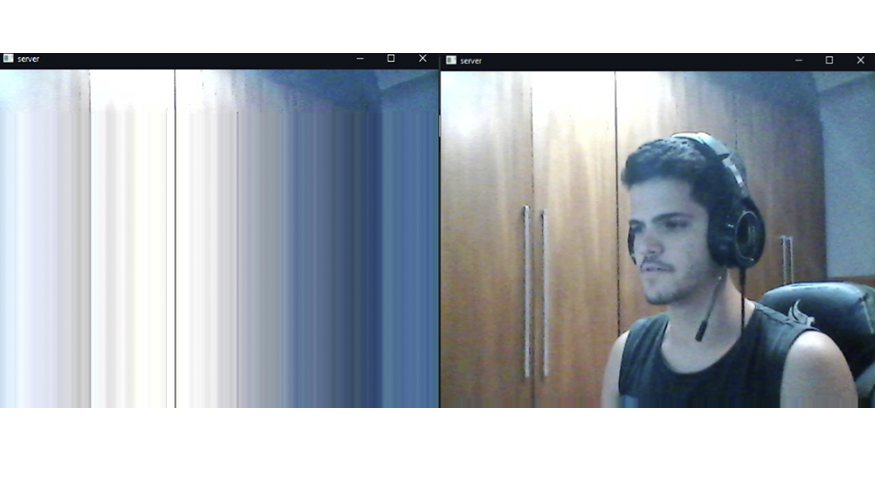
\includegraphics[width=.95\linewidth]{figuras/header.png}
%     \caption{Comparação entre uma imagem defeituosa e imagem corrigida com o \textit{header}.}
%     \label{fig:header}
%         \end{subfigure}
%         \begin{subfigure}{.45\textwidth}
%             \centering
%             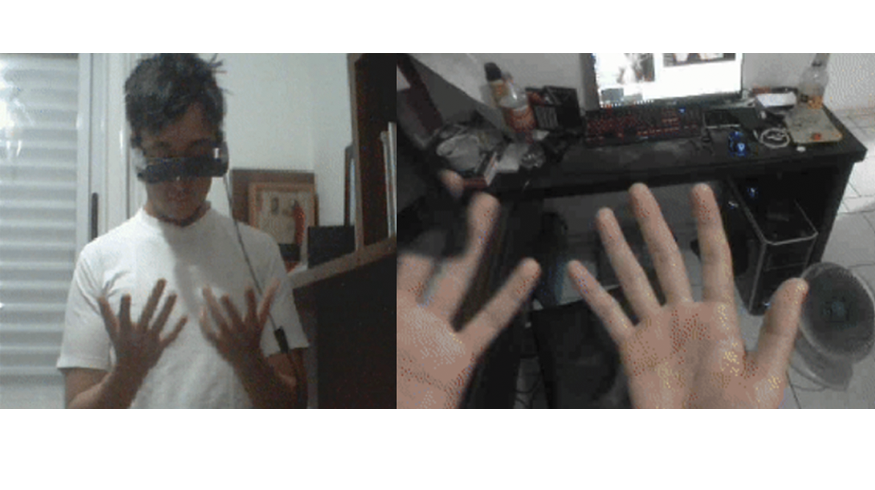
\includegraphics[width=.95\linewidth]{figuras/comm.png}
%             \caption{Êxito na transmissão em tempo real das imagens dos óculos para o computador.}
%             \label{fig:communication}
%         \end{subfigure}
%         \caption{Resultados dos testes de comunicação Fonte: Autor.}
%         \label{fig:comm-tests}
% \end{figure}

% % \begin{figure}[ht]
% %     \centering
% %     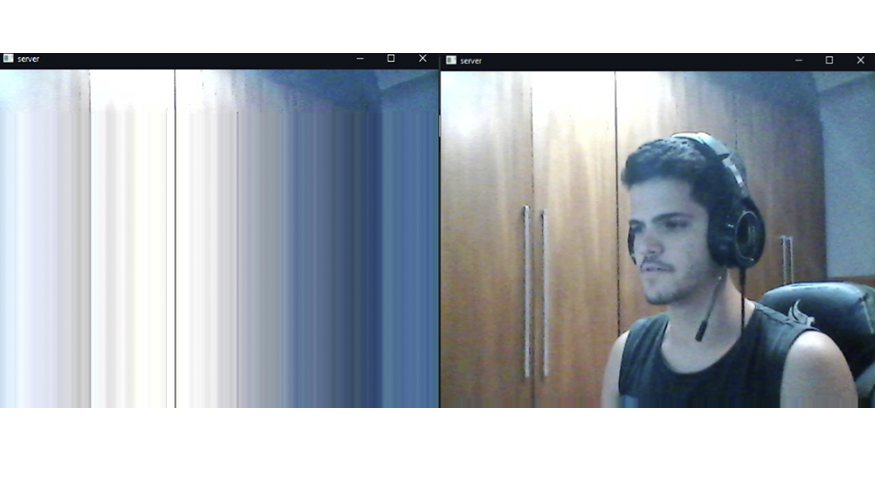
\includegraphics[width=.6\linewidth]{figuras/header.png}
% %     \caption{(A) Falha na transmissão\(\,\)(B) Imagem real. Fonte: Autor.}
% %     \label{fig:header}
% % \end{figure}

% % \begin{figure}[ht]
% %     \centering
% %     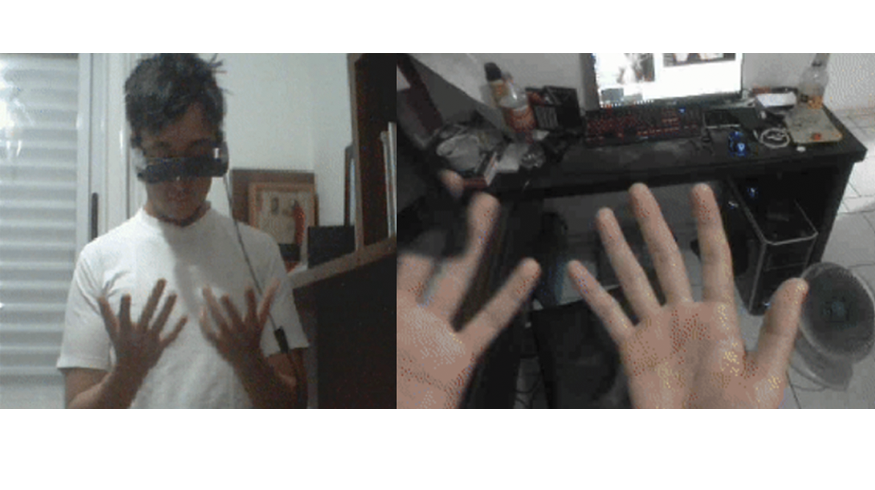
\includegraphics[width=.65\linewidth]{figuras/comm.png}
% %     \caption{Transmissão em tempo real das imagens dos óculos. Fonte: Autor.}
% %     \label{fig:communication}
% % \end{figure}

% A solução desse problema foi fazer um envio de uma mensagem de tamanho fixo (\textit{header}) informando ao computador o tamanho da próxima imagem, garantindo a captura completa da informação de cada foto (Figura \ref{fig:header}). Esse estudo e investigação do problema ampliou muito os conhecimentos de redes e seus protocolos de comunicação. Foi possível adquirir um resultado melhor que o esperado na transmissão de vídeo, obtendo uma taxa superior a 20 quadros por segundo, sua variação é sensível ao conteúdo da imagem por causar variação na taxa de compressão do formato \textit{JPEG} (\textit{Joint Photographic Experts Group}). 

% \subsection{Estimação da posição da projeção}

% A aplicação objetiva exibir os detalhes da anatomia cerebral de um paciente em AR para auxiliar os procedimentos operatórios de um neurocirurgião. Para isso, devemos utilizar um método que estime a relação entre o mundo real e virtual para sobrepormos a cabeça do paciente com a vista 3D dos seus dados da tomografia computadorizada. A procura desse método é o objeto de pesquisa de muitas referências bibliográficas. Nesse ponto da pesquisa, o projeto pode receber os métodos pesquisados por outros estudantes do laboratório, como a técnica de \textit{surface matching} da cabeça do paciente ou a estimação da posição corporal com \textit{machine learning}. No entanto, optamos por um método com baixa complexidade para darmos ênfase no objetivo de completarmos todo o sistema e, em um futuro breve, torná-lo em algo mais adequado para o ambiente cirúrgico.

% \begin{figure}[!h]
%     \centering
%     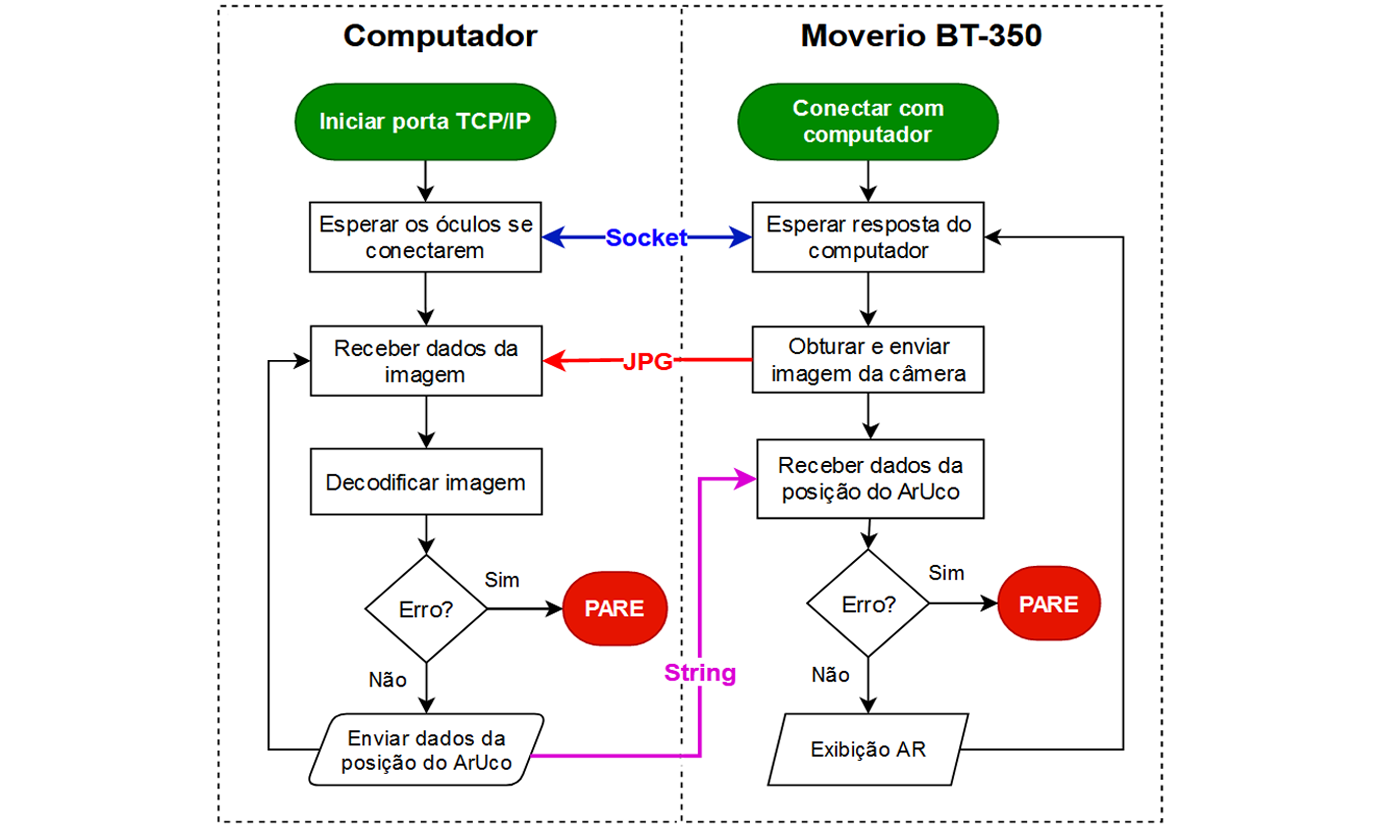
\includegraphics[width=.9\linewidth]{figuras/flowchart.png}
%     \caption{Fluxograma dos processos da execução do \textit{VCranium}. Fonte: Autor.}
%     \label{fig:flowchart}
% \end{figure}

% O método de estimação escolhido foi a detecção de marcadores fiduciais nativos da biblioteca do \textit{OpenCV}, o \textit{ArUco}. A estratégia de marcadores, especificamente os com forma quadrada, é comumente utilizada em aplicações de realidade aumentada pela sua rápida responsividade e robustez \cite{Romero-Ramirez2018}. Ele é especial por ter quatro pontos proeminentes (os quatro vértices) que facilitam sua detecção e seu conteúdo interno, preenchido com um padrão único que serve de identificador para o computador \cite{Poroykov2020}.

% O algoritmo da detecção \textit{ArUco} foi implementado junto ao programa \textit{Python} do computador. Esse módulo tem como entrada uma imagem dos óculos e saída as coordenadas da posição e rotação do marcador. Os dados são formatados em uma mensagem de tamanho fixo e enviado por \textit{TCP}, semelhante ao \textit{header} da imagem. Na rotina de execução dos óculos, ele primeiro obtura a imagem e envia para o computador, então ele espera a resposta com as informações do \textit{ArUco} correspondentes à imagem e por fim ele posiciona a projeção AR. Na detecção de quaisquer erros de formatação dos \textit{header}, são emitidos como erros fatais no programa, parando todos os processos da execução, vistos no fluxograma da figura \ref{fig:flowchart}.

% \subsection{Interface com usuário}

% Para a criação da interface, demos mais atenção ao funcionamento da projeção das imagens nas lentes dos óculos. A tecnologia empregada é a \textit{Si-OLED (Silicon - Organic Light-Emitting Diode)} que tem a característica de exibir os \textit{pixels} pretos como regiões desligadas de \textit{LED}, i.e, áreas escuras são regiões transparentes e áreas claras são regiões visíveis \cite{oculosspecs}. Pensando nisso, a interface apresenta as partes interativas mais claras, para chamar atenção do usuário, e um fundo preto para causar um efeito transparente (Figura \ref{fig:ui1}).

% % \begin{figure}[ht]
% %     \centering
% %         \begin{subfigure}{.45\textwidth}
% %             \centering
% %             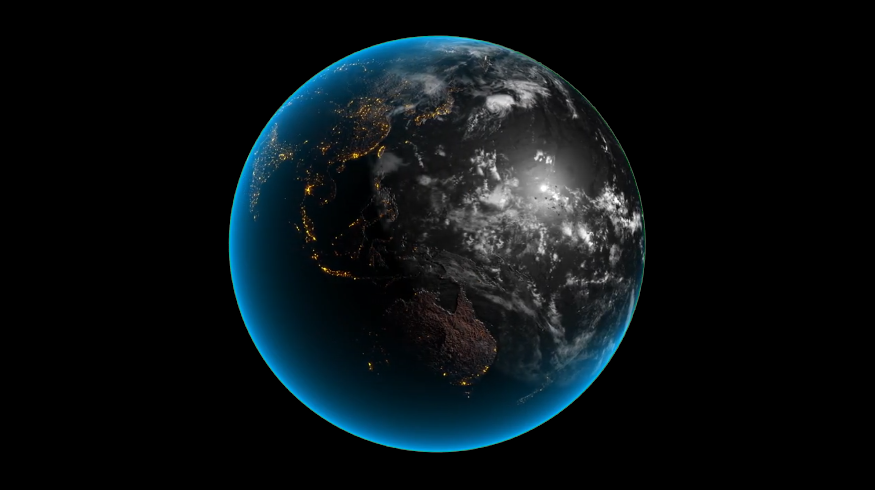
\includegraphics[width=.95\linewidth]{figuras/planeta.png}
% %             \caption{Imagem modificada com fundo preto.}
% %             \label{fig:planet}
% %         \end{subfigure}
% %         \begin{subfigure}{.45\textwidth}
% %             \centering
% %             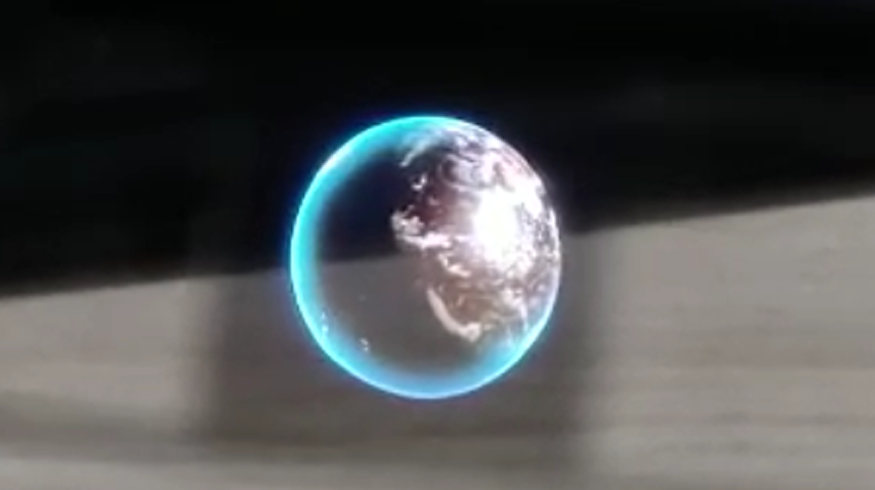
\includegraphics[width=.95\linewidth]{figuras/planetaAR.png}
% %             \caption{Exibição transparente nos óculos.}
% %             \label{fig:planetAR}
% %         \end{subfigure}
% %         \caption{As regiões escuras da imagem são vistos como transparência no \textit{display} dos óculos. Ilustração obtida de \cite{planet}. Fonte: Autor.}
% %         \label{fig:transparente}
% % \end{figure}

% \begin{figure}[ht]
%     \centering
%         \begin{subfigure}{.45\textwidth}
%             \centering
%             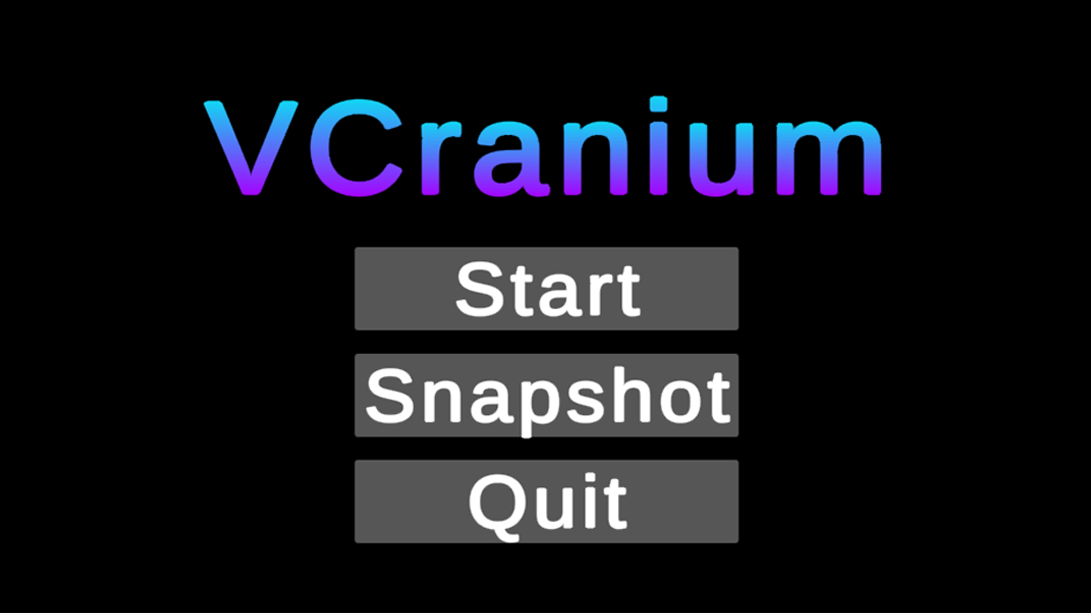
\includegraphics[width=.95\linewidth]{figuras/vcranium_main.png}
%             \caption{Menu principal do programa}
%             \label{fig:vcranium-connect}
%         \end{subfigure}
%         \begin{subfigure}{.45\textwidth}
%             \centering
%             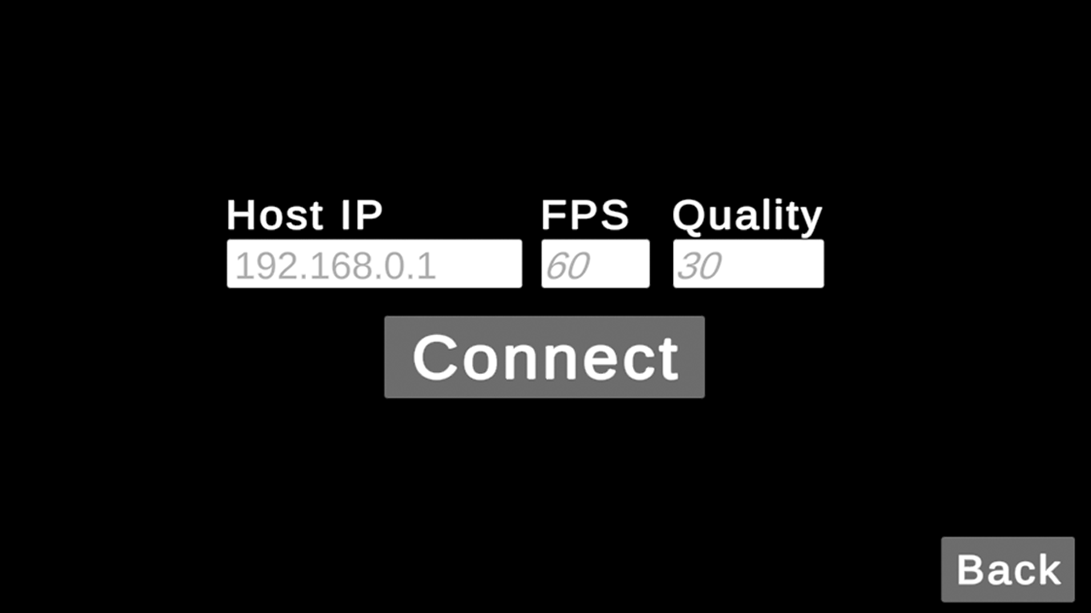
\includegraphics[width=.95\linewidth]{figuras/vcranium_connect.png}
%             \caption{Tela de conexão com computador}
%             \label{fig:vcranium2-connect}
%         \end{subfigure}
%         \caption{Imagens da interface do \textit{VCranium}. Fonte: Autor.}
%         \label{fig:ui1}
% \end{figure}

